% ===================================================================
%  Week 6 — Session 2: The Frequency Domain (applications & depth)
% ===================================================================
\documentclass[10pt,aspectratio=169]{beamer}
% ===================================================================
%  Shared Beamer preamble for "Practical Image Processing"
%  English slides. Compile with pdfLaTeX.
% ===================================================================

\usetheme{metropolis}
\usepackage[T1]{fontenc}
\usepackage[utf8]{inputenc}
\usepackage{lmodern}
\usepackage{listings}
\usepackage{tcolorbox}
\usepackage{fontawesome5}
\usepackage{booktabs}
\usepackage{amsmath,amssymb}
\usepackage{tikz}
\usepackage{pgfplots}
\pgfplotsset{compat=1.17}
\usetikzlibrary{arrows.meta,positioning,shapes.geometric,fit,backgrounds,matrix}
\tcbuselibrary{skins,breakable}

% ---- Palette --------------------------------------------------------
\definecolor{coursePrimary}{HTML}{1B4965}   % deep blue
\definecolor{courseAccent}{HTML}{E76F51}    % coral
\definecolor{courseGood}{HTML}{2A9D8F}      % teal
\definecolor{courseBad}{HTML}{C0392B}       % red
\definecolor{courseInfo}{HTML}{2980B9}      % blue
\definecolor{codeBg}{HTML}{F5F6FA}
\definecolor{codeKw}{HTML}{8E44AD}
\definecolor{codeStr}{HTML}{2A9D8F}
\definecolor{codeCom}{HTML}{7F8C8D}

\setbeamercolor{frametitle}{bg=coursePrimary}
\setbeamercolor{progress bar}{fg=courseAccent}
\setbeamercolor{alerted text}{fg=courseAccent}
\metroset{block=fill,sectionpage=progressbar,numbering=fraction}

% ---- Code listings (Python is built into listings) -----------------
\lstdefinestyle{course}{
  backgroundcolor=\color{codeBg},
  basicstyle=\ttfamily\scriptsize,
  keywordstyle=\color{codeKw}\bfseries,
  stringstyle=\color{codeStr},
  commentstyle=\color{codeCom}\itshape,
  numberstyle=\tiny\color{codeCom},
  numbers=left, numbersep=6pt,
  showstringspaces=false, breaklines=true, breakatwhitespace=true,
  tabsize=4, columns=fullflexible,
  frame=single, framesep=4pt, rulecolor=\color{gray!30},
  keepspaces=true, upquote=true, language=Python,
}
\lstset{style=course}
\lstdefinelanguage{bash}{
  keywords={cd,pip,python,venv,source,import}, sensitive=true,
  morecomment=[l]{\#}, morestring=[b]', morestring=[b]",
}

% ---- Reusable callout boxes ----------------------------------------
\newtcolorbox{goodbox}[1][Good practice]{colback=courseGood!8,colframe=courseGood,
  fonttitle=\bfseries,title={\faCheck~#1},boxrule=0.6pt,left=4pt,right=4pt,top=3pt,bottom=3pt}
\newtcolorbox{badbox}[1][Pitfall]{colback=courseBad!8,colframe=courseBad,
  fonttitle=\bfseries,title={\faTimes~#1},boxrule=0.6pt,left=4pt,right=4pt,top=3pt,bottom=3pt}
\newtcolorbox{infobox}[1][Note]{colback=courseInfo!8,colframe=courseInfo,
  fonttitle=\bfseries,title={\faInfoCircle~#1},boxrule=0.6pt,left=4pt,right=4pt,top=3pt,bottom=3pt}
\newtcolorbox{mathbox}[1][Math]{colback=coursePrimary!6,colframe=coursePrimary,
  fonttitle=\bfseries,title={\faCalculator~#1},boxrule=0.6pt,left=4pt,right=4pt,top=3pt,bottom=3pt}

\newcommand{\keyidea}[1]{\begin{alertblock}{Key idea}#1\end{alertblock}}
\newcommand{\term}[1]{\textbf{\color{coursePrimary}#1}}
\newcommand{\code}[1]{\lstinline[basicstyle=\ttfamily\small]|#1|}

% ---- A helper to draw a small pixel grid, cells shaded by value ----
% \pixelgrid{ {10,20,120,200,240}, {30,60,130,180,230}, ... }
\newcommand{\pixelgrid}[1]{%
  \begin{tikzpicture}[font=\scriptsize,scale=0.6]
    \foreach \row [count=\ry] in {#1} {
      \foreach \val [count=\cx] in \row {
        \draw[gray,fill=coursePrimary!8] (\cx,-\ry) rectangle ++(1,-1);
        \node at (\cx+0.5,-\ry-0.5) {\val};
      }
    }
  \end{tikzpicture}}


\title{The Frequency Domain}
\subtitle{Week 6 — Session 2: Periodic noise, phase \& the transform family}
\author{Practical Image Processing}
\date{Lecture 6.2 \textbullet\ 60--70 min}

\begin{document}

\maketitle

\begin{frame}{Recap of Session 1}
  \begin{columns}[T]
    \begin{column}{0.58\textwidth}
      \begin{itemize}
        \item Every image is a \term{sum of 2D sinusoids}; the DFT re-describes it on frequency axes.
        \item We read spectra: centre = DC, directions = perpendicular bright lines, off-centre
              peaks = repeating structure.
        \item We filtered by \term{masking}: low/high-pass, ideal vs smooth (ringing).
      \end{itemize}
    \end{column}
    \begin{column}{0.42\textwidth}
      \begin{alertblock}{Today}
        The pay-off: kill \term{periodic noise} with a notch, understand \term{phase}, meet the
        \term{FFT}, \term{DCT} and \term{wavelets}, and see \term{aliasing} + lighting in frequency.
      \end{alertblock}
    \end{column}
  \end{columns}
\end{frame}

\begin{frame}{Roadmap}\tableofcontents\end{frame}

% ==================================================================
\section{Periodic noise \& notch filtering}
% ==================================================================

\begin{frame}{Periodic noise: the killer app}
  \begin{columns}[T]
    \begin{column}{0.33\textwidth}\begin{center}
      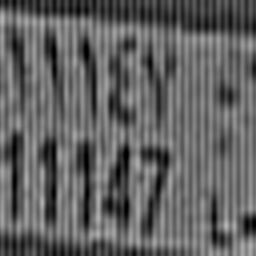
\includegraphics[width=\linewidth]{../assets/periodic_noisy.png}\\{\scriptsize striped noise}
    \end{center}\end{column}
    \begin{column}{0.33\textwidth}\begin{center}
      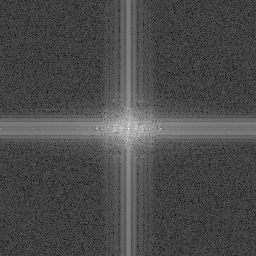
\includegraphics[width=\linewidth]{../assets/periodic_spectrum.png}\\{\scriptsize spectrum: 2 bright peaks}
    \end{center}\end{column}
    \begin{column}{0.33\textwidth}\begin{center}
      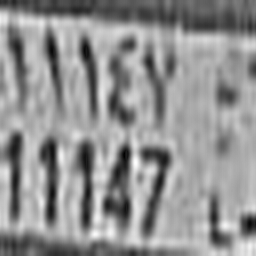
\includegraphics[width=\linewidth]{../assets/periodic_fixed.png}\\{\scriptsize after notch: clean}
    \end{center}\end{column}
  \end{columns}
  \vspace{3pt}
  \keyidea{Repeating stripes are a nightmare in the spatial domain — but two dots in frequency.
  Zero the dots (a \term{notch} filter), invert, done.}
\end{frame}

\begin{frame}{Where do the two peaks come from?}
  \begin{mathbox}
    A pure stripe pattern is a cosine:
    $\;n(x,y)=A\cos\!\big(2\pi(u_0 x + v_0 y)\big)$.\\[2pt]
    Euler: $\cos\theta = \tfrac12(e^{j\theta}+e^{-j\theta})$.
  \end{mathbox}
  \begin{itemize}
    \item So a single cosine is exactly \term{two} complex exponentials, at $+(u_0,v_0)$ and $-(u_0,v_0)$.
    \item In the spectrum that is two bright \term{deltas}, symmetric about the centre.
    \item Higher stripe frequency $\rightarrow$ peaks sit farther from the centre.
  \end{itemize}
  \keyidea{Every periodic pattern lands on a small number of isolated points. That is exactly why
  it is easy to remove here and impossible to remove pixel-by-pixel.}
\end{frame}

\begin{frame}{Notch filtering}
  \begin{itemize}
    \item A \term{notch} filter zeroes small regions of the spectrum (the noise peaks) and keeps the rest.
    \item Find the peaks (they're symmetric about the centre), mask them, inverse-transform.
    \item Perfect for scan lines, halftone patterns, sensor interference — real document artifacts.
  \end{itemize}
  \begin{goodbox}
    For DocScan: if a scanned form has a repeating background pattern, a notch filter removes it cleanly.
  \end{goodbox}
\end{frame}

\begin{frame}{Worked example: locating a peak}
  \begin{mathbox}
    Image $512\times512$, centred spectrum. A stripe repeats every \term{8 px} horizontally.
    Cycles across the width: $512/8 = 64$.
  \end{mathbox}
  \begin{itemize}
    \item The peak sits $64$ px left \emph{and} right of centre on the horizontal axis:
          columns $256\pm64 = 192$ and $320$, row $256$.
    \item A finer stripe (every 4 px) $\rightarrow 128$ cycles $\rightarrow$ peaks at $\pm128$ — farther out.
    \item Mask a small disc (radius $\sim3$--$5$ px) at \emph{both} points, then invert.
  \end{itemize}
  \keyidea{Peak distance from centre $=$ image size $\div$ stripe period. Always notch the symmetric
  partner too, or you re-inject the stripe.}
\end{frame}

\begin{frame}[fragile]{Notch filter in code}
\begin{lstlisting}[language=Python]
F = np.fft.fftshift(np.fft.fft2(noisy))
mag = 20*np.log(np.abs(F) + 1)             # inspect to find peaks
H, W = noisy.shape; cy, cx = H//2, W//2
Y, X = np.ogrid[:H, :W]
notch = np.ones((H, W))
for (py, px) in [(cy, cx+64), (cy, cx-64)]:  # both symmetric peaks
    D = np.sqrt((X-px)**2 + (Y-py)**2)
    notch[D <= 4] = 0                        # zero a small disc
clean = np.abs(np.fft.ifft2(np.fft.ifftshift(F * notch)))
\end{lstlisting}
  \code{fft2} $\rightarrow$ zero the peak discs $\rightarrow$ \code{ifft2}. Same three-step workflow, targeted mask.
\end{frame}

\begin{frame}{Notch vs band-reject}
  \begin{columns}[T]
    \begin{column}{0.5\textwidth}\begin{center}
      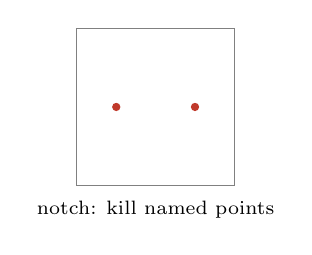
\begin{tikzpicture}[scale=0.5]
        \draw[gray] (0,0) rectangle (4,4);
        \fill[courseBad] (1,2) circle (3pt);
        \fill[courseBad] (3,2) circle (3pt);
        \node at (2,-0.6){\scriptsize notch: kill named points};
      \end{tikzpicture}
    \end{center}\end{column}
    \begin{column}{0.5\textwidth}\begin{center}
      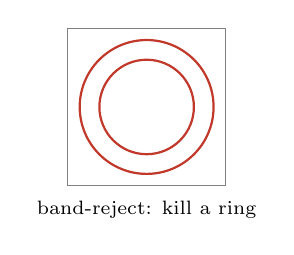
\begin{tikzpicture}[scale=0.5]
        \draw[gray] (0,0) rectangle (4,4);
        \draw[courseBad,thick] (2,2) circle (1.2);
        \draw[courseBad,thick] (2,2) circle (1.7);
        \node at (2,-0.6){\scriptsize band-reject: kill a ring};
      \end{tikzpicture}
    \end{center}\end{column}
  \end{columns}
  \vspace{4pt}
  \begin{itemize}
    \item \term{Notch}: remove a few specific frequencies — best when you can see the peaks.
    \item \term{Band-reject}: remove an annulus of frequencies — when noise fills a whole ring
          (e.g. a rotationally-symmetric texture).
  \end{itemize}
\end{frame}

% ==================================================================
\section{Amplitude vs phase}
% ==================================================================

\begin{frame}{Amplitude vs phase}
  \begin{itemize}
    \item The DFT has \term{magnitude} (how much of each frequency) and \term{phase} (where it sits).
    \item Surprising fact: \term{phase} carries most of the \emph{structure} — swap two images' phases and you swap what you see.
    \item We visualize magnitude, but don't forget phase exists and matters.
  \end{itemize}
  \begin{mathbox}
    $F(u,v)=|F(u,v)|\,e^{\,j\phi(u,v)}$ — amplitude $|F|$ and phase $\phi$ together carry the full image.
  \end{mathbox}
\end{frame}

\begin{frame}{The phase-swap thought experiment}
  \begin{center}
  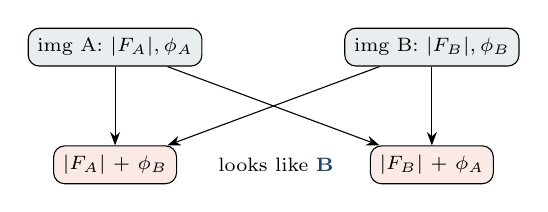
\begin{tikzpicture}[node distance=6mm,font=\scriptsize]
    \node[draw,rounded corners,fill=coursePrimary!10] (a) {img A: $|F_A|,\phi_A$};
    \node[draw,rounded corners,fill=coursePrimary!10,right=18mm of a] (b) {img B: $|F_B|,\phi_B$};
    \node[draw,rounded corners,fill=courseAccent!15,below=10mm of a] (c) {$|F_A|$ + $\phi_B$};
    \node[draw,rounded corners,fill=courseAccent!15,below=10mm of b] (d) {$|F_B|$ + $\phi_A$};
    \draw[-{Stealth}] (a) -- (c); \draw[-{Stealth}] (b) -- (c);
    \draw[-{Stealth}] (a) -- (d); \draw[-{Stealth}] (b) -- (d);
    \node[right=4mm of c,text width=3.2cm] {looks like \term{B}};
  \end{tikzpicture}
  \end{center}
  Combine A's amplitude with B's phase and you \emph{see} B. Edges and object positions live in the
  \term{phase}; the amplitude mostly sets contrast per frequency.
\end{frame}

% ==================================================================
\section{The FFT \& the transform family}
% ==================================================================

\begin{frame}{FFT: why it's fast}
  \begin{itemize}
    \item A naive DFT is $O(N^2)$; the \term{Fast Fourier Transform} is $O(N\log N)$.
    \item This is what makes frequency-domain filtering practical on real images.
    \item Numpy/OpenCV give you the FFT; you just prepare the mask and invert.
  \end{itemize}
  \begin{mathbox}
    For a $1024^2$ image, FFT is $\sim$50{,}000$\times$ fewer operations than the naive sum.
  \end{mathbox}
\end{frame}

\begin{frame}{Worked example: counting the savings}
  \begin{mathbox}
    Treat the image as $N=1024^2\approx 10^6$ samples. Naive DFT $\approx N^2$; FFT $\approx N\log_2 N$.
  \end{mathbox}
  \begin{itemize}
    \item Naive: $(10^6)^2 = 10^{12}$ operations.
    \item FFT: $10^6 \times 20 = 2\times10^7$ operations.
    \item Ratio: $10^{12}/(2\times10^7) = 5\times10^4$ — the $\sim$50{,}000$\times$ speed-up.
  \end{itemize}
  \keyidea{The FFT is not a different transform — it is the \emph{same} DFT computed cleverly by
  reusing shared sub-sums. Without it the frequency domain would be a textbook curiosity.}
\end{frame}

\begin{frame}{Other transforms: the DCT (JPEG)}
  \begin{columns}[T]
    \begin{column}{0.55\textwidth}
      \begin{itemize}
        \item \term{DCT} (cosine transform): the heart of JPEG.
        \item Split the image into $8\times8$ blocks; transform each; keep the low-frequency
              coefficients, quantize the rest away.
        \item Real photos concentrate energy in the top-left of the block $\rightarrow$ big compression.
      \end{itemize}
    \end{column}
    \begin{column}{0.45\textwidth}\begin{center}
      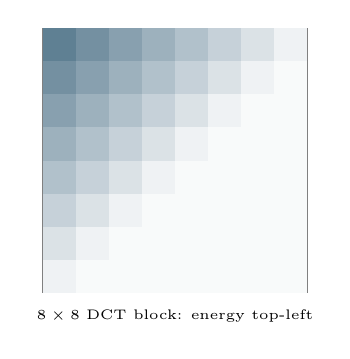
\begin{tikzpicture}[scale=0.42,font=\tiny]
        \draw[step=1,gray] (0,0) grid (8,8);
        \foreach \i in {0,...,7}{\foreach \j in {0,...,7}{
          \pgfmathsetmacro{\d}{\i+\j}
          \pgfmathsetmacro{\g}{max(3, 70-9*\d)}
          \fill[coursePrimary!\g] (\j,7-\i) rectangle ++(1,1);}}
        \node at (4,-0.7){$8\times8$ DCT block: energy top-left};
      \end{tikzpicture}
    \end{center}\end{column}
  \end{columns}
  \begin{infobox}
    JPEG's blocking artifacts are exactly these $8\times8$ blocks becoming visible when you quantize
    too hard.
  \end{infobox}
\end{frame}

\begin{frame}{Other transforms: wavelets}
  \begin{itemize}
    \item \term{Wavelets}: multi-scale, localized in \emph{both} space and frequency.
    \item Fourier tells you \emph{which} frequencies exist but not \emph{where}; wavelets keep some
          spatial location at each scale.
    \item Great for \term{denoising} (shrink small coefficients) and compression (JPEG-2000).
  \end{itemize}
  \begin{mathbox}
    Uncertainty trade-off: you cannot be perfectly sharp in both position \emph{and} frequency —
    each transform picks a point on that curve.
  \end{mathbox}
\end{frame}

% ==================================================================
\section{Aliasing \& lighting}
% ==================================================================

\begin{frame}{Aliasing, in the frequency view}
  \begin{columns}[T]
    \begin{column}{0.55\textwidth}
      \begin{itemize}
        \item Sampling \term{replicates} the spectrum on a grid.
        \item If the spectrum is too wide, the copies \term{overlap} — high frequencies fold into
              low ones.
        \item That fold-over is the moir\'e / jaggies you saw in Week 1.
      \end{itemize}
    \end{column}
    \begin{column}{0.45\textwidth}\begin{center}
      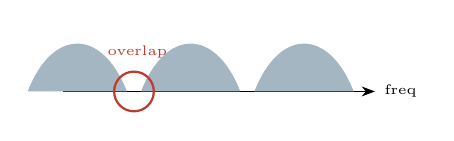
\begin{tikzpicture}[scale=0.9,font=\tiny]
        \draw[-{Stealth}] (-0.2,0) -- (4.2,0) node[right]{freq};
        \foreach \c in {0,1.6,3.2}{
          \fill[coursePrimary!40] (\c,0) ++(-0.7,0)
            .. controls (\c-0.35,0.9) and (\c+0.35,0.9) .. (\c+0.7,0);}
        \node[courseBad] at (0.85,0.55){overlap};
        \draw[courseBad,thick] (0.8,0) circle (0.28);
      \end{tikzpicture}\\{\scriptsize spectral copies overlapping}
    \end{center}\end{column}
  \end{columns}
\end{frame}

\begin{frame}{Anti-aliasing = narrow the spectrum first}
  \begin{itemize}
    \item Blur (\term{low-pass}) before downsampling so the spectrum is narrow enough that copies
          don't overlap.
    \item This is the frequency-domain reason for the ``blur then resize'' rule from Week 1.
    \item The cutoff should be the \term{Nyquist} frequency of the target resolution.
  \end{itemize}
  \begin{goodbox}
    When shrinking a meter photo, always apply a Gaussian pre-filter — otherwise the digit edges
    alias into false patterns that wreck OCR.
  \end{goodbox}
\end{frame}

\begin{frame}{Homomorphic filtering}
  \begin{itemize}
    \item Uneven lighting is low-frequency; reflectance (the content) is higher-frequency.
    \item Take the \code{log}, then high-pass slightly to suppress illumination and boost detail.
    \item Useful for a document photographed under a gradient of light — flattens the shading.
  \end{itemize}
  \begin{goodbox}
    Another DocScan trick: homomorphic filtering can even out lighting before thresholding.
  \end{goodbox}
\end{frame}

\begin{frame}{The homomorphic pipeline}
  \begin{center}
  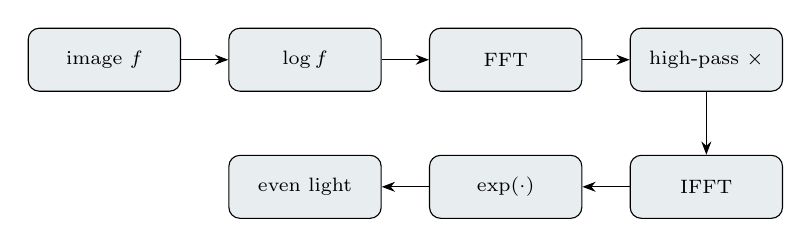
\begin{tikzpicture}[node distance=6mm,font=\scriptsize,
      box/.style={draw,rounded corners,fill=coursePrimary!10,minimum height=8mm,text width=1.7cm,align=center}]
    \node[box] (a) {image $f$};
    \node[box,right=of a] (b) {$\log f$};
    \node[box,right=of b] (c) {FFT};
    \node[box,right=of c] (d) {high-pass $\times$};
    \node[box,below=8mm of d] (e) {IFFT};
    \node[box,left=of e] (f) {$\exp(\cdot)$};
    \node[box,left=of f] (g) {even light};
    \draw[-{Stealth}] (a)--(b); \draw[-{Stealth}] (b)--(c); \draw[-{Stealth}] (c)--(d);
    \draw[-{Stealth}] (d)--(e); \draw[-{Stealth}] (e)--(f); \draw[-{Stealth}] (f)--(g);
  \end{tikzpicture}
  \end{center}
  The \code{log} turns the \emph{product} illumination$\times$reflectance into a \emph{sum}, so a linear
  high-pass can separate them. Then \code{exp} undoes the log.
\end{frame}

% ==================================================================
\section{In-class exercise}
% ==================================================================

\begin{frame}{\faPen~In-class exercise (10 min)}
  \begin{infobox}[Design a notch]
  \end{infobox}
  A $256\times256$ scan has diagonal stripes repeating every $\sim 16$ px along the diagonal.
  \begin{enumerate}
    \item How many cycles fit across the image along that diagonal?
    \item Roughly where (relative to centre) do the two peaks appear?
    \item What radius would you give each notch disc, and why not larger?
    \item Why must you zero both symmetric peaks?
  \end{enumerate}
\end{frame}

\begin{frame}{\faPen~Debrief}
  \begin{itemize}
    \item (1) Diagonal length $\approx 256\sqrt2\approx362$ px; $362/16\approx 23$ cycles.
    \item (2) Two peaks on the \emph{diagonal} through the centre, $\sim 23$ units out each way
          (perpendicular to the stripes' direction).
    \item (3) A small radius ($3$--$5$ px): large enough to cover the blob, small enough to keep
          nearby real content.
    \item (4) The spectrum is conjugate-symmetric; leaving the partner re-creates a (weaker) real
          cosine and the stripe returns.
  \end{itemize}
  \keyidea{Notch design is geometry: period $\rightarrow$ distance, direction $\rightarrow$ angle,
  always in symmetric pairs.}
\end{frame}

% ==================================================================
\section{When to use it \& wrap-up}
% ==================================================================

\begin{frame}{When to use frequency vs spatial}
  \begin{itemize}
    \item \term{Frequency}: periodic noise, very large filters, analyzing texture/orientation.
    \item \term{Spatial}: local operations, edges, morphology, anything position-dependent.
    \item Most day-to-day work is spatial; frequency is the right tool for specific jobs.
  \end{itemize}
  \keyidea{Don't reach for the FFT by default — but when you see a repeating pattern, it's exactly the tool.}
\end{frame}

\begin{frame}{Frequency thinking $\rightarrow$ deep learning}
  \begin{itemize}
    \item CNNs learn spatial kernels, but the frequency view explains what they capture (edges = high-freq).
    \item Some modern architectures operate partly in frequency for efficiency.
    \item Understanding frequency deepens your intuition for what any filter — hand-made or learned — does.
  \end{itemize}
\end{frame}

\begin{frame}{What you should now be able to do}
  \begin{itemize}
    \item Remove periodic noise with a notch filter — locate peaks from the stripe period.
    \item Explain amplitude vs phase, and why phase holds the structure.
    \item Reason about the FFT's speed and place it among DCT / wavelets.
    \item See aliasing and uneven lighting as frequency-domain phenomena.
  \end{itemize}
\end{frame}

\begin{frame}{Pitfalls recap}
  \begin{badbox}
    \begin{itemize}
      \item Notching only one of the symmetric peaks — the stripe comes back.
      \item Over-large notch discs — you delete real detail with the noise.
      \item Forgetting the \code{log} in homomorphic filtering — illumination stays multiplicative.
      \item Downsampling without a pre-blur — aliasing folds high frequencies into your image.
    \end{itemize}
  \end{badbox}
\end{frame}

\begin{frame}{This week's deliverable}
  \begin{alertblock}{Due before Week 7 (see \code{project/})}
    \begin{enumerate}
      \item Compute and display the magnitude spectrum of 3 real images; interpret each.
      \item Implement low-pass and high-pass by masking; compare to spatial blur/edges.
      \item Add periodic (stripe) noise; locate the peaks; remove it with a notch filter.
      \item Show the notch peak coordinates you used and how you derived them from the stripe period.
      \item Note: when is frequency-domain the right tool for a DocScan problem, and when not?
    \end{enumerate}
  \end{alertblock}
\end{frame}

\begin{frame}[standout]
  An image is a sum of waves.\\[4pt]
  \normalsize Some problems that are impossible in space are trivial in frequency.
\end{frame}

\end{document}
